\documentclass[12pt, letterpaper]{article}
\usepackage{graphicx} %LaTeX package to import graphics
\graphicspath{{images/}} %configuring the graphicx package

\title{
    
\includegraphics[scale=0.5]{unibalogo.jpg}~\\[1cm]
    \textbf{Sviluppo di un contatore elettrico intelligente}
}
\author{Stefano Antonio Labianca}

\date{22 Gennaio 2024}
\renewcommand*\contentsname{Tabella dei contenuti}
\renewcommand{\figurename}{Figura}

\begin{document}

\maketitle


\textbf{matricola: } 758364
\hfill
\textbf{email: } s.labianca10@studenti.uniba.it

\par\noindent\rule{\textwidth}{0.4pt}~\\[5cm]

\tableofcontents ~\\[5cm]

\section{Introduzione}

Nell'arco della nostra giornata, usiamo diversi dispositivi elettronici e,
alle volte, anche per diverse ore della giornata o addirittura per tutto
il giorno. \\ \break
Per chi abita nelle zone di campagna, o in abitazioni singole, usare molti
dispositivi elettronici contemporaneamente, specialmente se hanno alti consumi o
possiedono una classe energetica bassa, fa scattare il salvavita.

\subsection{Dispositivo salvavita}

Il "salvavita", o più propriamente detto interruttore differenziale, è un dispositivo
che arresta il flusso di energia elettrica dal contatore di
un'abitazione, proteggendo persone e animali. \\ \break
Questi interruttori, monitorano la differenza di corrente in entrata
e in uscita dal dispositivo e, quando la differenza di corrente in entrata e in
uscita supera una certa soglia, allora l'interruttore scatta togliendo l'alimentazione
al circuito.

\begin{figure}
    \centering
    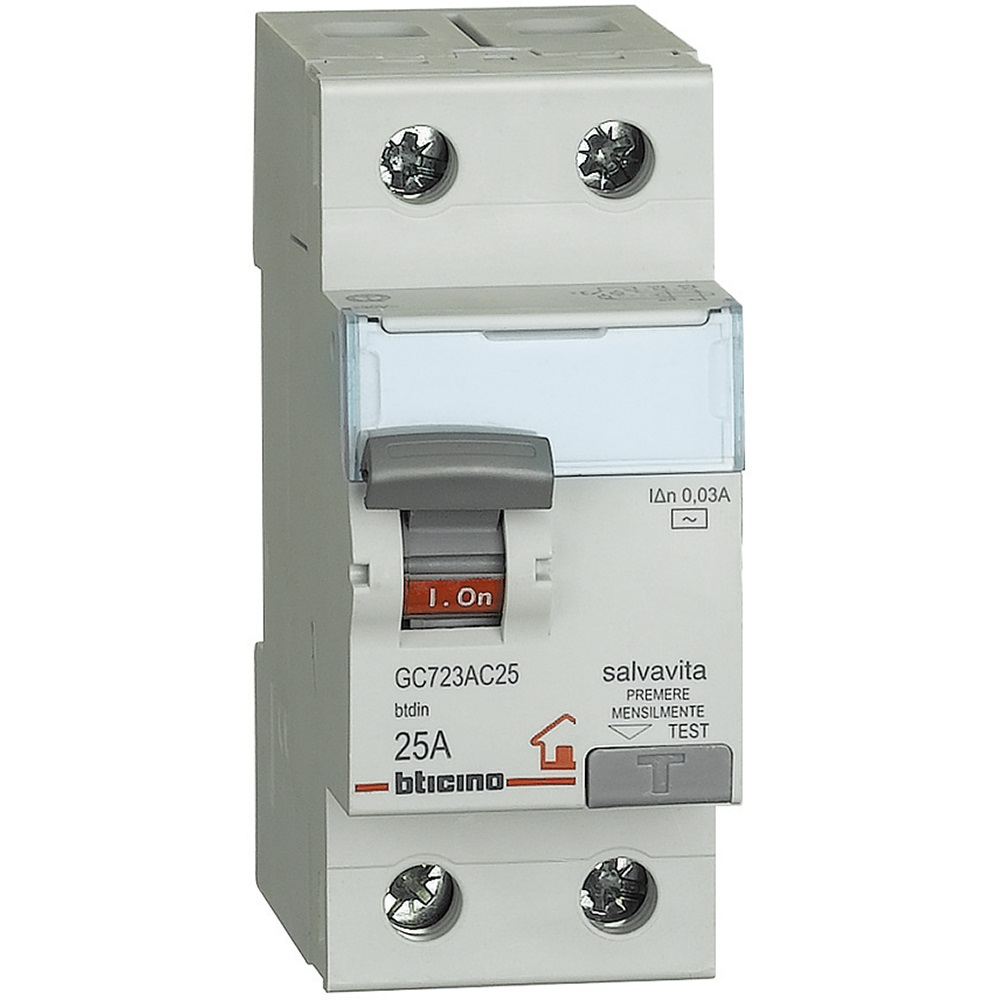
\includegraphics[scale=0.2]{interruttore-diff.jpg}
    \caption{Esempio di contatore differenziale}
\end{figure}


\subsection{Obiettivo del progetto}

Il progetto si pone l'obiettivo di sviluppare un programma in grado di svolgere
i seguenti task:

\begin{enumerate}
    \item Determinare da una lista di dispositivi, quali possono tenere accesi contemporaneamente
          senza che salti il salvavita.
    \item Tenere traccia dei dispositivi elettronici e del loro consumo in Watt.
    \item Ottenere tutti quei dispositivi che rispettano certi vincoli di consumo energetico.
\end{enumerate}





% \section{CSP}

% \section{Ontologie}


% \section{Sistema esperto}

% \section{Sviluppi futuri}

\end{document}